\section{Grundlagen} % (fold)
\label{sec:grundlagen}

	\subsection{Begriffe}
	\label{sub:begriffe}
		\subsubsection{Pattern und Antipattern} % (fold)
		\label{ssub:pattern_und_anti_pattern}
			"`Entwurfsmuster (englisch design patterns) sind bewährte Lösungsschablonen für wiederkehrende Entwurfsprobleme sowohl in der Architektur als auch in der Softwarearchitektur und -entwicklung. Sie stellen damit eine wiederverwendbare Vorlage zur Problemlösung dar, die in einem bestimmten Zusammenhang einsetzbar ist."'\autocite{pattern15}
			\\
			"`Während "`Design Patterns"' in der Software-Entwicklung allgemein übliche und bekannte Ansätze sind, um Probleme zu lösen, sind Anti-Patterns Negativ-Beispiele – die zeigen, wie man es nicht macht - von bereits durchgeführten, gescheiterten Projekten, die dem erkennenden Mitarbeiter zielgerichtete Hinweise darauf geben, wie die Aufgabenstellung besser gelöst werden könnte. Als Synonym ist auch der Begriff Negativmuster im Gebrauch. Es ist tatsächlich möglich, daß das, was gestern noch als allgemein gangbarer Lösungsweg bezeichnet wurde, heute schon ein "`Antipattern"' ist [...]"' \autocite{Stepken06}

		% subsubsection pattern_und_anti_pattern (end)

		\subsubsection{TTFB} % (fold)
		\label{ssub:ttfb}
		TTFB ist die Abkürzung für "`Time to first byte"'. Dieser Begriff beschreibt den Prozess: Sende eine Anfrage an den Server mittels HTTP Protokoll, baue eine Verbindung zum Server auf, verarbeite diese Anfrage und sende die Antwort zurück. Die Zeit bis der Browser das erste byte der Antwort erhält, ist die TTFB.
		% subsubsection ttfb (end)

		\subsubsection{RTT} % (fold)
		\label{ssub:rtt}
			Round Trip Time wird im Deutschen Paketumlaufzeit genannt. Es bezeichnet die Zeit die ein Datenpaket braucht um in einem Netzwerk von Sender A zu Empfänger B und wieder zurück zu gelangen.
		% subsubsection rtt (end)

		\subsubsection{Above The Fold} % (fold)
		\label{ssub:above_the_fold}
			\begin{figure}[htbp]
				\begin{center}
					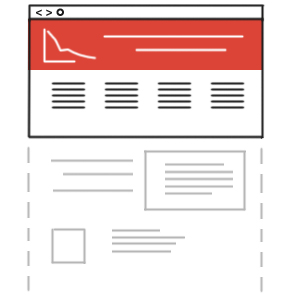
\includegraphics[width=0.3\textwidth]{above_the_fold.jpg}
					\caption{Darstellung des sichtbaren Bereichs vor dem Scrollen}
					\label{fig:above_the_fold}
				\end{center}
			\end{figure}
			
			Damit ist der auf einem Bildschirm sichtbare Bereich vor dem Scrollen gemeint. Diesem Bereich wird eine besondere Wichtigkeit zugesprochen.

			\begin{quote}
				 \textit{"`In an analysis of 57,453 eyetracking fixations, we found that there was a dramatic drop-off in user attention at the position of the page fold. Elements above the fold were seen more than elements below the fold: the 100 pixels just above the fold were viewed 102\% more than the 100 pixels just below the fold."'} \autocite{nng15}
			\end{quote}

			Wichtige Informationen oder Navigationselemente sind meistens dort zu finden. Eine Webseite die nach dem Paradigma des Responsive-Webdesign aufgebaut ist kann dabei 3 oder mehrere Ansichten haben die alle einen unterschiedlichen "`above the fold"' bereich haben. Eine Anwendung kann aber auch unterschiedliche Seiten haben, auf dem der Anwender beim Aufrufen der Seite landen kann. Zum Beispiel wenn dieser An- oder Abgemeldet ist. Paradebeispiel dafür sind Facebook oder Twitter.
		% subsubsection above_the_fold (end)

		\subsubsection{Kritischer Rendering-Pfad} % (fold)
		\label{ssub:critical_render_path}
			Auf Englisch "`critical render path"' genannt, ist der wohl wichtigste Begriff, wenn es um schnelle Ladezeiten geht. Durch die Optimierung des Rendering Pfads kann die benötigte Zeit für das erste Rendern der Seite erheblich verkürzt werden. Das Verständnis des Rendering-Pfads ist zudem eine Voraussetzung für die Erstellung von schnellen Webanwendungen und soll in diesem Abschnitt ausführlich erklärt werden.\\

			Wie kann der Browser eine Webanwendung rendern?

			\begin{itemize}
				\item Nach dem Seitenaufruf läd der Browser die HTML Datei vom Server.
				\item Der Browser liest das HTML und sieht nach, ob zusätzliche Ressourcen benötigt werden (zum Beispiel Bilder, Javascript oder Stylesheets).
				\item Diese Ressourcen werden angefragt 
			\end{itemize}

			\begin{figure}[htbp]
				\begin{center}
					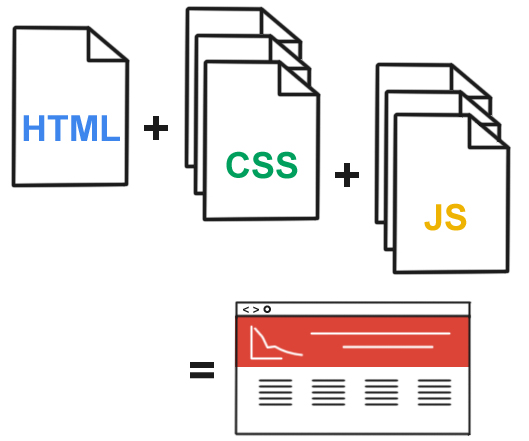
\includegraphics[width=0.4\textwidth]{critical_render_path.jpg}
					\caption{Ressourcen die für das Rendern von nöten sind}
					\label{fig:critical_render_path}
				\end{center}
			\end{figure}

			Kritischer Rendering-Pfad (engl. Critical Render path) bezeichnet die für den Browser nötigen Ressourcen um die aufgerufene Seite zu zeichnen.

			Dazu zählt auch das Übersetzen ("`Parsing"' genannt) des HTML Dokuments, das Ausführen von Javascript und das Anfragen von nötigen externen Ressourcen. Als Ressourcen zählen: Bilder, Javascript, Stylesheets und XHR\footnote{XMLHttpRequest (XHR) ist eine Programmierschnittstelle für JavaScript zum Übertragen von Daten über das HTTP-Protokoll. XMLHttpRequest bildet einen Grundbaustein der Ajax-Technik.\autocite{xhr15}}.\\

			Mehr dazu wird in Abschnitt \ref{..fehlt} erläutert.
			% todo: ref fehlt

		% subsubsection critical_render_path (end)
	
	% subsection begriffe (end)

	\subsection{Latenz}
	\label{sub:latenz}
		TCP Handshake
		TCP Slowstart
		Http/1.1
		Payload
		RTT
		Einfluss der Datenrate auf die Geschwindigkeit

		
	% subsection latenz (end)

	
% section grundlagen (end)